Nesse capítulo são apresentados conceitos que servem de base para o desenvolvimento do presente trabalho. Inicialmente será brevemente abordada a história do Controle Ótimo para que, em seguida, o problema de Controle Ótimo seja definido. Em seguida, apresenta-se uma visão geral sobre os Métodos Diretos, empregados nos pacotes avaliados no presente trabalho. Por fim, esses pacotes são brevemente apresentados. 
\section{Uma breve história do Controle Ótimo}

\todo[inline, color=pink]{Histórico do Controle Ótimo}

O Controle Ótimo (CO) é um conjunto de métodos que possibilita a determinação das trajetórias de estados e controles que, quando impostas a um dado sistema dinâmico, garantem que as restrições operacionais associadas ao mesmo sejam satisfeitas, enquanto promovem a minimização (ou maximização) de um dado índice de desempenho \cite{kirk_optimal_2004, becerra_optimal_2008, kelly_introduction_2017}. As origens do CO remontam ao ano de 1697, quando Johann Bernoulli, professor de matemática da Universidade de Groningen, no norte da Holanda, publicou a solução do problema da braquistócrona \cite{sussmann_300_1997}, proposto por Galileo Galilei 59 anos antes \cite{bryson_optimal_1996}. Em 1696, Johann Bernoulli desafiou seus contemporâneos a resolver esse problema, que consiste na determinação da trajetória a ser percorrida por uma esfera que deve se mover entre dois pontos A e B, apenas sob a ação da gravidade, no menor tempo possível, conforme ilustrado na Figura \ref{fig:revisao:braquistocrona}. Soluções para o problema da braquistócrona foram propostas por Johan Bernoulli, Newton, Leibniz, l'Hopital e Jakob Bernoulli, irmão de Johan \cite{bryson_optimal_1996}.

\noindent	
\begin{minipage}{\textwidth}
	\vspace{\onelineskip}
	\centering
	\includegraphics[width=0.5\linewidth]{draw/revisao/pdf/braq}
	\captionof{figure}[Representação do problema da braquistócrona]{Representação do problema da braquistócrona.}
	\label{fig:revisao:braquistocrona}
	\vspace{\onelineskip}
\end{minipage}

Pode-se dizer que o CO é uma extensão do Cálculo de Variações (CV), desenvolvido por Isaac Newton em 1685, e que buscava determinar o formato da ponta de um projétil que levasse à minimização do arrasto aerodinâmico. Em 1744, Leonard Euler publicou um livro intitulado \textit{\textcolor{red}{Arthur, colocar aqui o nome do livro em inglês, por favor}}, no qual são apresentadas as bases para o desenvolvimento teórico do CV. Euler e Jean Louis Lagrange trocaram cartas a respeito desse livro e juntos desenvolveram a equação de Euler-Lagrange. Esta descreve a condição necessária de primeira ordem associada à solução de um problema de CV \cite{bryson_optimal_1996}.

Em 1836, Willian Rowan Hamilton publicou um trabalho aplicando o CV ao projeto de sistemas mecânicos a partir da minimização da força exercida pelos mesmos. As soluções obtidas por Hamilton foram baseadas na resolução de duas equações diferenciais, e por esse motivo, o autor foi criticado, em 1838, por Karl Gustav Jacob Jacobi, que afirmou que apenas uma equação bastaria. A partir do trabalho desses dois autores desenvolveu-se a equação de Hamilton-Jacobi, que serviu de base para que Richard Bellman propusesse a programação dinâmica mais de 100 anos depois \cite{bryson_optimal_1996}. 

Com base no trabalho desenvolvido por Karl Wilhelm Theodor Weierstrass no final do século XIX, Oskar Bolza e Gilbert A. Bliss associaram ao CV o rigor matemático que o acompanha até os dias atuais. A partir do trabalho atribuído a Bolza e Bliss, McShane desenvolveu, em 1939, um método para resolução de problemas de CV, que seria estendido por Pontryagin anos depois dando origem ao princípio do mínimo de Pontryagin. Em 1957, Placido Cicala escreveu uma monografia a respeito do emprego do CV no desenvolvimento de projetos de engenharia e, em 1963, Derek Lawden foi o primeiro a empregar o CV na determinação de trajetórias para veículos espaciais \cite{bryson_optimal_1996}. 

No entanto, é importante salientar que o Controle Clássico também serviu de base para o desenvolvimento do CO. O Controle Clássico consiste num conjunto de metologias normalmente baseadas em procedimentos a partir dos quais determinam-se os ganhos de um controlador para que a implementação do mesmo leve a uma resposta em malha fechada satisfatória \cite{bryson_optimal_1996}.

Durante e após a Segunda Guerra Mundial, diversos métodos baseados nas transformadas de Laplace e Fourier, e nas variáveis complexas, foram desenvolvidos para que o desempenho e a estabilidade de sistemas de controle em malha fechada fossem previstos. Com o surgimento dessas técnicas, critérios quantitativos passaram a ser definidos no domínio da frequência, como os ganhos de margem e de fase, e no domínio do tempo, como o tempo de acomodação e o máximo sobressinal (ou \textit{overshoot}) associados à resposta do sistema a uma entrada do tipo degrau \cite{bryson_optimal_1996}.

A utilização da integral do quadrado do erro (ISE) na sintonização de um controlador em malha fechada foi proposta pela primeira vez por Newton, Gould e Kaiser em 1957. Já em 1961, Chang propôs o projeto de um controlador com base em restrições associadas à integral do quadrado da ação de controle. Em 1960, Kalman estabeleceu os conceitos de variáveis de estado e controle, que são largamente utilizadas no CO, assim como um índice de desempenho integral computado a partir das magnitudes dos controles e erros. Kalman mostrou, empregando o CV, que os controles poderiam ser determinados a partir de uma realimentação linear das variáveis de estado. Posteriormente, o controlador proposto por Kalman seria chamado de Regulador Linear Quadrático (LQR) \cite{bryson_optimal_1996}. 

Por fim, é preciso ressaltar que o CO possui também origens na Programação Não Linear (PNL), desenvolvida logo após a Segunda Guerra Mundial. Esta consiste na otimização de uma dada função objetivo a partir da determinação de parâmetros (ou variáveis de projeto), sujeitos a restrições de igualdade e desigualdade. Caso o perfil de controle seja aproximado por um conjunto finito de pontos no tempo, é possível que a PNL seja empregada na determinação do valor assumido pelo esforço de controle em cada um desses pontos, de forma que o problema de OC inicialmente proposto seja resolvido de forma numérica \cite{bryson_optimal_1996}. Esse abordagem será discutida em detalhes mais adiante uma vez que serve de base para o desenvolvimento do presente trabalho.  

\section{O problema de Controle Ótimo}

%\todo[inline, color=pink]{Definição do Controle Ótimo}
%
%O CO consiste em um conjunto de metodologias que possibilita a determinação de perfis de controles e estados, ou de ganhos de controladores em malha fechada, que minimizem um dado índice de desempenho de forma que sejam respeitadas restrições diferenciais referentes à dinâmica do sistema a ser controlado \cite{bryson_optimal_1996}. Além das restrições dinâmicas, é importante salientar que, em alguns casos, é preciso que sejam consideradas restrições de caminho, associadas à evolução temporal dos estados e/ou controles, restrições terminais, relacionadas aos valores assumidos pelos estados ao fim da trajetória, e restrições associadas especificamente às amplitudes dos estados e/ou controles \cite{becerra_optimal_2008}.

\todo[inline, color=pink]{O Problema de Controle Ótimo}

O problema de Controle Ótimo (PCO) é definido de acordo com a formulação de Bolza \cite{becerra_optimal_2008}:
%
\begin{subequations}
\begin{equation}
	\label{eq:revisao:PCO}
		\underset{\mathbf{u}(t)}{\text{min}} \; J = \varphi \big( \mathbf{x}(t_f), t_f \big) + \int_{t_0}^{t_f} L \big( \mathbf{x}(t), \mathbf{u}(t), t \big) \, dt
\end{equation}
\vspace{-0.4cm}
\begin{equation}
		\mathbf{\dot{x}}(t) = \mathbf{f} \big( \mathbf{x}(t), \mathbf{u}(t), t \big), \; \mathbf{x}(t_0) = \mathbf{x_0} 
\end{equation}
\end{subequations}
%
sendo $ \mathbf{x}(t) $ e $ \mathbf{u}(t) $, respectivamente, os vetores de estados e controles do sistema, $ t $ a variável temporal, $ t_0 $ e $ t_f $ os tempo inicial e final, respectivamente, $ J $ o funcional a ser minimizado (ou maximizado), também chamado índice de desempenho ou função objetivo, $ \varphi $ a função de custo terminal, também conhecida como função de Mayer, $ L $ a função de custo de caminho, também intitulada função de Lagrange, $ \mathbf{f} $ o sistema de equações que descreve a dinâmica do sistema, tipicamente no espaço de estados, e $ \mathbf{x_0} $ a condição inicial atribuída a $ \mathbf{x}(t) $. Considera-se que estão associados à formulação de $ \mathbf{f} $ $ n $ estados e $ m $ controles, de forma que:
%
\begin{subequations}
\begin{equation}
\mathbf{x}(t) = \begin{bmatrix} x^{(1)}(t) & x^{(2)}(t) & \dots & x^{(n)}(t) \end{bmatrix}^T
\end{equation}
\vspace{-0.5cm}
\begin{equation}
\mathbf{u}(t) = \begin{bmatrix} u^{(1)}(t) & u^{(2)}(t) & \dots & u^{(m)}(t) \end{bmatrix}^T
\end{equation}
\end{subequations}

Vale ressaltar que caso $ t_0 $ e $ t_f $ não sejam previamente estabelecidos, devem ser determinados por meio da resolução do PCO, e nesse caso, restrições associadas aos limites de $ t_0 $ e $ t_f $ devem ser consideradas. Além disso, uma vez determinado $ \mathbf{u}(t) $, é possível que, de posse de $ \mathbf{x_0} $, determinem-se a trajetórias dos estados com base na computação de $ \mathbf{f} \big( \mathbf{x}(t), \mathbf{u}(t), t \big) $.

A formulação de um PCO pode incluir restrições associadas às amplitudes dos estados e/ou controles, que serão referenciadas ao longo do texto como restrições laterais: 
%
\begin{subequations}
\begin{equation}
\mathbf{x_L} \leq \mathbf{x}(t) \leq \mathbf{x_U} 
\end{equation}
\vspace{-0.75cm}
\begin{equation}
\mathbf{u_L} \leq \mathbf{u}(t) \leq \mathbf{u_U}
\end{equation}
\end{subequations}
sendo os índices $ L $ e $ U $ utilizados na representação dos limites inferiores e superiores dos estados e controles. Além disso, podem-se considerar restrições de caminho, associadas à evolução temporal dos estados e/ou controles, 
%
\begin{equation}
	\mathbf{c}(\mathbf{x}(t), \mathbf{u}(t), t) \leq \mathbf{0} 
\end{equation}
%
e restrições terminais, relacionadas aos valores assumidos pelos estados ao fim da trajetória,
%
\begin{equation}
	{\bm \psi}(\mathbf{x}(t_f), t_f) \leq \mathbf{0} 
\end{equation}
%
sendo $ \mathbf{c} $ e $ {\bm \psi} $, funções quaisquer.  

Um PCO pode ser formulado, por exemplo, para que os perfis de velocidade $ x_2(t) $ e posição $ x_1(t) $ de um carro que corre sobre um trilho sejam determinadas. Para tanto, é necessário que seja também computado o perfil da força $ u(t) $ exercida sobre o carro, representado nesse caso como um ponto de massa. Pode-se considerar ainda que o tempo despendido na transposição de 10 m de trilho, e a força empregada na realização desse movimento devam ser minimizados. Supondo que, devido aos materiais utilizados na construção do aparato em questão, e do motor que movimenta carro, haja limitações na velocidade e na potência associadas à movimentação do mesmo, pode-se determinar $ x_1(t) $, $ x_2(t) $, $ u(t) $ e $ t_f $ a partir da resolução do PCO introduzido como segue:
%
\begin{subequations}
\begin{equation}
\label{eq:revisao:PCOExemplo}
\underset{\mathbf{u}(t), \, t_f}{\text{min}} \; J = t_f + \int_{0}^{t_f} u^2(t) \, dt
\end{equation}
\vspace{-0.3cm}
\begin{equation}
\dot{x}_1(t) = x_2(t), \; x_1(0) = 0 \text{ m} 
\end{equation}
\vspace{-0.6cm}
\begin{equation}
\dot{x}_2(t) = u(t), \; x_2(0) = 0 \text{ m$/$s} 
\end{equation}
\vspace{-0.6cm}
\begin{equation}
-2 \text{ m$/$s} \leq x_2(t) \leq 2 \text{ m$/$s} 
\end{equation}
\vspace{-0.6cm}
\begin{equation}
-10 \text{ N} \leq u(t) \leq 10 \text{ N} 
\end{equation}
\vspace{-0.6cm}
\begin{equation}
-15 \text{ W} \leq u(t) \, x_2(t) \leq 15 \text{ W} 
\end{equation}
\vspace{-0.6cm}
\begin{equation}
x_1(t_f) = 10 \text{ m}
\end{equation}
\end{subequations}

A formulação do PCO apresentada contempla uma restrição de caminho vinculada à potência empregue na movimentação do carro, uma restrição terminal relacionada à posição final do mesmo, e restrições associadas a limitações na velocidade $ x_2(t) $ do carro e na força $ u(t) $ que atua sob o mesmo. 

\todo[inline, color=pink]{Conceitos Gerais}

\section{Conceitos Gerais}

A presente seção tem por objetivo apresentar uma série de conceitos importantes para o estudo do PCO. Neste caso, são avaliadas características que abrangem uma equação algébrico-diferencial - EAD (resultante da aplicação de otimalidade para o PCO), bem como aspetos relacionados com a presença de restrições \cite{bryson_optimal_1996,lobato2004}.

\begin{itemize}

\item Arcos Singulares: arcos onde a matriz de derivadas segundas da função  Hamiltoniano com relação às variáveis de controle é singular. Neste contexto, alguns PCOs são definidos a partir de domínios nos quais podem ser observadas regiões em que a condição estacionária $ \mathbf{H_{u}} = \partial \mathit{H} / \partial u $ é satisfeita ao mesmo tempo em que a matriz Hessiana $ \mathbf{H_{uu}} = \partial^2 \mathit{H} / \partial u^2 $ associada ao Hemiltoniano $ \mathit{H} $ é singular. Essas regiões são chamadas arcos singulares, e nelas, $ u(t) $ não pode ser unicamente definido pela condição estacionária, sendo necessário impor que as derivadas temporais de $ \mathbf{H_{u}} $ sejam nulas ao longo do arco. Adversidades numéricas podem ser enfrentadas caso métodos computacionais sejam empregados na resolução de PCOs que possuam arcos singulares \cite{betts_practical_2001, becerra_optimal_2008}.

Como exemplos de PCOs que apresentam arcos singulares pode-se citar: 
%
\begin{itemize}
	\item Determinação de trajetórias ótimas para foguetes de sondagem, que realizam voos suborbitais para coleta de dados utilizados em estudos meteorológicos e astronômicos \cite{nasa_what_2004};
	
	\item Estabelecimento do curso de uma aeronave que realiza voos periódicos para minimização do gasto de combustível \cite{speyer_periodic_1996};
	
	\item Estudo da influência do fenômeno meteorológico \textit{wind shear}, que consiste na variação brusca da direção e/ou velocidade do vento, no pouso de uma aeronave \cite{anac_wind_2018}.
\end{itemize}

\item Condição de Canto: ponto onde ocorre descontinuidade no perfil de controle ou na inclinação das trajetórias das variáveis de estado. 

\item EAD com Índice Superior e Redução de Índice: são as equações com índice maior do que $1$. O índice diferencial é o número mínimo de vezes que o sistema de equações algébrico-diferenciais ou parte dele deve ser diferenciado com relação ao tempo para determinar transformá-lo em um puramente diferencial. Este conceito representa uma medida da dificuldade de solução de sistema de EADs, decorrente de mau condicionamento, instabilidade, singularidade e má convergência. Do ponto de vista da solução numérica é desejável que o índice das EADs seja o menor possível devido à dificuldade associada na solução deste em comparação com a solução de equações diferenciais ordinárias com rigidez numérica. Entretanto,
esta redução obtida através da simples diferenciação das restrições pode não satisfazer as restrições originais de maneira exata, com sérias implicações quando elas envolvem propriedades físicas importantes. Portanto, devem ser consideradas formas de reintroduzir restrições perdidas no sistema, chamadas invariantes.

\item Eventos: pontos de junção entre os arcos sujeitos a restrições e os arcos sem
restrições.

\item Funções Identificadoras de Fase: relação matemática obtida a partir da aplicação da condição de otimalidade em um PCO e que tem por finalidade indicar a ativação o não de uma restrição. Um caso particular e de grande interesse é quando a variável de controle aparece linearmente na função Hamiltoniano. 

\end{itemize}

\todo[inline, color=pink]{Métodos Diretos}

\section{Métodos Diretos}

Os métodos empregados na resolução de PCOs podem ser divididos em duas principais categorias: os Métodos Indiretos e os Métodos Diretos. Os Métodos Indiretos se baseiam na resolução das condições necessárias de otimalidade associadas ao PCO. A formulação dessas condições depende da definição do Hamiltoniano $\mathit{H} \big( \mathbf{x}(t), \mathbf{u}(t), {\bm \lambda}(t), t \big)$: 
%
\begin{equation}
	\mathit{H} \big( \mathbf{x}(t), \mathbf{u}(t), {\bm \lambda}(t), t \big) = L \big( \mathbf{x}(t), \mathbf{u}(t), t \big) + {\bm \lambda}^T(t) \; \mathbf{f} \big( \mathbf{x}(t), \mathbf{u}(t), t \big)
\end{equation}
%
em que $ {\bm \lambda}(t) $ são os multiplicadores de Lagrange, também conhecidos como co-estados ou variáveis adjuntas. Assim sendo, as condições de otimalidade, ou equações de Euler-Lagrange, são introduzidas como segue \cite{becerra_optimal_2008}.
%
\begin{subequations}
\begin{equation}
	\label{eq:revisao:condicoesOtimalidade}
		{\bm \dot{ \bm \lambda}}^T(t) = - \frac{\partial \mathit{H} \big( \mathbf{x}(t), \mathbf{u}(t), {\bm \lambda}(t), t \big)}{\partial \mathbf{x}(t)}
\end{equation}
\vspace{-0.2cm}
\begin{equation}
	{\bm \lambda}^T(t_f) = \frac{\partial \varphi \big( \mathbf{x}(t_f), t_f \big)}{\partial \mathbf{x}(t)} \Biggr|_{t = t_f}
	\end{equation}
\begin{equation}
\label{eq:revisao:condicoesOtimalidadeb}
		\frac{\partial \mathit{H} \big( \mathbf{x}(t), \mathbf{u}(t), {\bm \lambda}(t), t \big)}{\partial \mathbf{u}(t)} = \mathbf{0}
\end{equation}
\end{subequations}

Apesar das soluções obtidas por meio dos Métodos Indiretos serem comumente bastante acuradas, pode ser consideravelmente difícil, a depender do PCO em análise, formular as condições necessárias de otimalidade, algo que um usuário com pouco conhecimento da teoria do CO dificilmente seria capaz de fazer. Além disso, o sucesso dos métodos numéricos empregados na resolução do sistema descrito pela Eqs. \eqref{eq:revisao:condicoesOtimalidade}-\eqref{eq:revisao:condicoesOtimalidadeb} depende fortemente das estimativas iniciais atribuídas a $ {\bm \lambda}(t) $, que não podem ser determinados de forma intuitiva, uma vez que não possuem significado físico \cite{betts_practical_2001}. 

Já os Métodos Diretos são baseados na discretização dos estados e controles, de forma que a resolução do PCO se dê a partir da determinação dos valores atribuídos aos mesmos em pontos específicos da trajetória, denominados nós (ou pontos) de colocação, conforme observado na Figura \ref{fig:revisao:discretizacao}. Mais de 90\% dos pacotes computacionais desenvolvidos para a resolução de PCOs são baseados nos Métodos Diretos. Essa popularidade se deve à existência de inúmeros pacotes robustos e bem estabelecidos para solução de um problema de programação não linear (PPNL), capazes de lidar de forma simples e direta com restrições de igualdade e desigualdade, e que não requerem que as equações associadas aos co-estados sejam fornecidas pelo usuário \cite{biral_notes_2016}. 

Uma vez que os estados, os controles, a função objetivo e as restrições associadas à dinâmica do PCO, tenham sido discretizados de forma que:
%
\begin{subequations}
\begin{equation}
t \rightarrow t_0, \, \dots, \, t_k, \, \dots, \, t_{M} 
\end{equation}
\vspace{-0.85cm}
\begin{equation}
\mathbf{x}(t) \rightarrow \mathbf{x}_0, \, \dots, \, \mathbf{x}_k, \, \dots, \, \mathbf{x}_{M}
\end{equation}
\vspace{-0.75cm}
\begin{equation}
\mathbf{u}(t) \rightarrow \mathbf{u}_0, \, \dots, \, \mathbf{u}_k, \, \dots, \, \mathbf{u}_{M}
\end{equation}
\end{subequations}
%
sendo $ \xi_k $ o valor atribuído à variável $ \xi $ no nó de colocação $ k $, é possível que o PCO em análise seja tratado como um problema de otimização clássica, mais especificamente um PPNL. Cabe ressaltar que $ M $ é o índice atribuído ao último nó de colocação, localizado em $ t = t_f $, e que, assumindo $ N $ como sendo o número de nós de colocação, tem-se $ M = N - 1 $. O processo de conversão de um PCO em um PPNL é conhecido como transcrição \cite{kelly_introduction_2017}. 

\begin{minipage}{\textwidth}
	\vspace{\onelineskip}
	\centering
	\includegraphics[width=0.7\linewidth]{draw/revisao/pdf/discretizacao}
	\captionof{figure}[Representação do processo de discretização em Métodos Diretos]{Representação do processo de discretização em Métodos Diretos.}
	\label{fig:revisao:discretizacao}
	\vspace{\onelineskip}
\end{minipage}

Os PPNLs são tipicamente formulados da seguinte maneira \cite{kelly_introduction_2017}, 
%
\begin{subequations}
\begin{equation}
\underset{\mathbf{z}}{\text{min}} \; F(\mathbf{z})
\end{equation}
\vspace{-0.75cm}
\begin{equation}
\mathbf{H}(\mathbf{z}) = \mathbf{0} 
\end{equation}
\vspace{-0.75cm}
\begin{equation}
\mathbf{G}(\mathbf{z}) \leq \mathbf{0}
\end{equation}
\vspace{-0.75cm}
\begin{equation}
\mathbf{z_L} \leq \mathbf{z} \leq \mathbf{z_U}
\end{equation} 
\end{subequations}
% 
em que $ F $ é o funcional a ser minimizado, $ \mathbf{H} $ e $ \mathbf{G} $ são os vetores de restrições de igualdade e desigualdade. Os limites inferior e superior associados ao vetor de variáveis de projeto (ou variáveis de decisão ou variáveis de busca) $ \mathbf{z} $, são denotados por $ \mathbf{z_L} $ e $ \mathbf{z_U} $ respectivamente.

Uma vez que o PPNL tenha sido resolvido e os valores atribuídos a $ \mathbf{x}(t) $ e $ \mathbf{u}(t) $ nos nós de colocação, denotados respectivamente por $ \mathbf{x}_k $ e $ \mathbf{u}_k $, tenham sido determinados, é possível que os perfis dos estados e controles sejam construídos a partir da interpolação de $ \mathbf{x}_k $ e $ \mathbf{u}_k $. A forma como se dá essa interpolação depende da metodologia empregada no processo de transcrição. As trajetórias dos controles, por exemplo, podem ser determinadas a partir da interpolação linear ou quadrática dos valores atribuídos a $ \mathbf{u}_k $, ao passo que as trajetórias dos estados podem ser especificadas com base na interpolação cúbica dos valores atribuídos a $ \mathbf{x}_k $ \cite{kelly_introduction_2017}. É possível ainda que as trajetórias de cada controle e estado sejam representadas por um único polinômio que percorra todos os nós de colocação \cite{becerra_psopt_2019}. 

%\subsection{Métodos de Colocação Direta}

%Como mencionado anteriormente, a transcrição de um PCO pode ser realizada de diversas maneiras. 

A implementação da maioria dos métodos de transcrição é baseada nos cinco passos listados a seguir:
%
\begin{enumerate}
	\item Discretização da integral associada à função objetivo;
	\item Discretização das restrições dinâmicas;
	\item Discretização das restrições de caminho, terminais e laterais;
	\item Solução do PPNL obtido a partir do processo de transcrição;
	\item Elaboração das trajetórias de estados e controles com base em $ \mathbf{x}_k $ e $ \mathbf{u}_k $ assumindo-se $ k = 0, \, 1, \, \dots, \, M $.
\end{enumerate}

A forma como cada uma dessas etapas será executada depende do método de transcrição adotado. Assim sendo, serão apresentados nas próximas seções alguns dos métodos mais comumente empregados na transcrição de PCOs.

\subsection{Colocação trapezoidal}
\label{sec:revisao:trap}

\todo[inline, color=pink]{Colocação trapezoidal}

A colocação trapezoidal é baseada na quadratura trapezoidal, empregada tanto na computação do integrando $L$ associada à função objetivo, quanto na discretização das restrições dinâmicas. Desta forma, assumindo-se $ h_k = t_{k+1} - t_k $, determina-se a integral de $L$ conforme a seguinte relação
%
\begin{equation}
	\label{eq:revisao:trap:integral}
	\int_{t_0}^{t_f} L \big( \mathbf{x}(t), \mathbf{u}(t), t \big) \, dt \approx \sum_{k=0}^{M-1} \frac{1}{2} h_k (L_k + L_{k+1})
\end{equation}
%
sendo $ L_k =  L \big( \mathbf{x}_k, \mathbf{u}_k, t_k \big)$ \cite{kelly_introduction_2017}.

Uma vez que os estados tenham sido discretizados é possível que as restrições diferenciais associadas à dinâmica do PCO sejam representadas por um conjunto de restrições algébricas. Para tanto, é necessário que as restrições dinâmicas sejam reescritas na forma integral e que a quadratura trapezoidal seja empregada \cite{kelly_introduction_2017}:
%
\begin{subequations}
\begin{equation}
\label{eq:revisao:trap:restricaoDinamica}
\mathbf{\dot{x}}(t) = \mathbf{f}(\mathbf{x}(t), \mathbf{u}(t), t)
\end{equation}
\vspace{-0.5cm}
\begin{equation}
\int_{t_k}^{t_{k+1}} \mathbf{\dot{x}}(t) \, dt = \int_{t_k}^{t_{k+1}} \mathbf{f}(\mathbf{x}(t), \mathbf{u}(t), t) \, dt
\end{equation}
\vspace{-0.25cm}
\begin{equation}
\mathbf{x}_{k+1} - \mathbf{x}_k \approx \frac{1}{2} h_k (\mathbf{f}_{k} + \mathbf{f}_{k+1})
\end{equation}
\end{subequations}

Assim sendo, $ M $ restrições de igualdade algébricas são formuladas a partir da equação anterior: 
%
\begin{equation}
	\mathbf{x}_{k+1} - \mathbf{x}_k - \frac{1}{2} \, h_k \, (\mathbf{f}_{k+1} + \mathbf{f}_k) = \mathbf{0}, \hspace{0.25cm} k = 0, \, \dots, \, M-1
\end{equation}
%
sendo $ \mathbf{f}_k = \mathbf{f}(\mathbf{x}_k, \mathbf{u}_k, t_k) $. Vale ressaltar que $ \mathbf{x}_k $ é uma variável de projeto, enquanto $ \mathbf{f}_k $ é obtido via avaliação do $ k $-ésimo nó de colocação  \cite{kelly_introduction_2017}.  

As restrições laterais, terminais e de caminho são incorporadas à formulação do PPNL a partir do momento em que são transformadas em restrições de igualdade e desigualdade. Infelizmente, uma vez que a resolução do PPNL depende apenas dos valores atribuídos aos estados e controles nos nós de colocação, somente nesses nós é possível garantir que as restrições serão de fato satisfeitas \cite{kelly_introduction_2017}. Assim sendo, as restrições associadas ao PCO podem ser transcritas da seguinte forma: 
%
\begin{subequations}
\begin{equation}
\mathbf{x_L} \leq \mathbf{x}(t) \leq \mathbf{x_U} \rightarrow \mathbf{x_L} \leq \mathbf{x}_k \leq \mathbf{x_U}, \; k = 0, \, \dots, \, M 
\end{equation}
\vspace{-0.85cm}
\begin{equation}
\mathbf{u_L} \leq \mathbf{u}(t) \leq \mathbf{u_U} \rightarrow \mathbf{u_L} \leq \mathbf{u}_k \leq \mathbf{u_U}, \; k = 0, \, \dots, \, M 
\end{equation}
\vspace{-0.7cm}
\begin{equation}
\mathbf{c}(\mathbf{x}(t), \mathbf{u}(t), t) \leq \mathbf{0} \rightarrow \mathbf{c}(\mathbf{x}_k, \mathbf{u}_k, t_k) \leq \mathbf{0}, \; k = 0, \, \dots, \, M
\end{equation}
\vspace{-0.7cm}
\begin{equation}
{\bm \psi}(\mathbf{x}(t_f), t_f) \leq \mathbf{0}  \rightarrow {\bm \psi}(\mathbf{x}_M, t_M) \leq \mathbf{0} 
\end{equation}
\end{subequations}
%
em que a condição inicial $ \mathbf{x_0} $ para o vetor de variáveis de estado é dado como:
%
\begin{equation}
	\mathbf{x}_k = \mathbf{x_0}, \hspace{0.25cm} k = 0 
\end{equation}
%

%As variáveis de projeto associadas ao PPNL advindo do processo de transcrição, considerando-se o caso geral em que $ t_0 $ e $ t_f $ devem ser determinados assim como $ \mathbf{u}_k $ e $ \mathbf{x}_k $, são introduzidas em \eqref{eq:revisao:variaveisPPNLTrap}
%%
%\begin{equation}
%	\label{eq:revisao:variaveisPPNLTrap}
%	\mathbf{z}^T = \begin{bmatrix} \mathbf{z_t}^T & \mathbf{z_x}^T & \mathbf{z_u}^T \end{bmatrix} 
%\end{equation}
%% 
%em que
%%
%\begin{equation}
%	\begin{gathered}
%		\mathbf{z_t}^T = \begin{bmatrix} t_0 & t_f \end{bmatrix} \\
%		\mathbf{z_x}^T = \begin{bmatrix} x^{(1)}_0 & x^{(1)}_1 & \dots & x^{(1)}_M & \dots & x^{(n)}_0 & x^{(n)}_1 & \dots & x^{(n)}_M \end{bmatrix} \\
%		\mathbf{z_u}^T = \begin{bmatrix} u^{(1)}_0 & u^{(1)}_1 & \dots & u^{(1)}_M & \dots & u^{(n)}_0 & u^{(n)}_1 & \dots & u^{(n)}_M \end{bmatrix} \\
%	\end{gathered}
%\end{equation}

Por fim, o emprego da colocação trapezoidal na avaliação do PCO descrito resulta no seguinte PPNL:
%
\begin{subequations}
\begin{equation}
\underset{\mathbf{u}_k, \, \mathbf{x}_k}{\text{min}} \; J = \varphi \big( \mathbf{x}_M, t_M \big) + \sum_{k=0}^{M-1} \frac{1}{2} h_k (L_k + L_{k+1}) \\
\end{equation}
\vspace{-0.1cm}
\begin{equation}
\mathbf{x}_{k+1} - \mathbf{x}_k - \frac{1}{2} \, h_k \, (\mathbf{f}_{k+1} + \mathbf{f}_k) = \mathbf{0}, \hspace{0.25cm} k = 0, \, \dots, \, M-1
\end{equation}
\vspace{-0.7cm}
\begin{equation}
\mathbf{x}(t_0) = \mathbf{x_0}
\end{equation}
\vspace{-0.7cm}
\begin{equation}
\mathbf{x_L} \leq \mathbf{x}_k \leq \mathbf{x_U}, \hspace{0.25cm} k = 0, \, \dots, \, M
\end{equation}
\vspace{-0.7cm}
\begin{equation}
\mathbf{u_L} \leq \mathbf{u}_k \leq \mathbf{u_U}, \hspace{0.25cm} k = 0, \, \dots, \, M
\end{equation}
\vspace{-0.7cm}
\begin{equation}
\mathbf{c}(\mathbf{x}_k, \mathbf{u}_k, t_k) \leq \mathbf{0} \hspace{0.25cm} k = 0, \, \dots, \, M \end{equation}
\vspace{-0.7cm}
\begin{equation}
{\bm \psi}(\mathbf{x}_M, t_M) \leq \mathbf{0} 
\end{equation}
\end{subequations}
%
em que $ t_0 $ e $ t_f $ são conhecidos. Não sendo esse o caso, $ t_0 $ e $ t_f $ devem ser determinadas de forma que as seguintes restrições sejam respeitadas:
%
\begin{subequations}
\begin{equation}
t_{0L} \leq t_0 \leq t_{0U}
\end{equation}
\vspace{-0.95cm}
\begin{equation}
t_{fL} \leq t_f \leq t_{fU}
\end{equation} 
\end{subequations}
%
sendo os limites inferiores de $ t_0 $ e $ t_f $ denotados por $ t_{0L} $ e $ t_{fL} $ e os superiores por $ t_{0U} $ e $ t_{fU} $, respectivamente. 

Uma vez que o PPNL tenha sido resolvido e que tanto $ \mathbf{x}_k $ quanto $ \mathbf{u}_k $ tenham sido determinados para $ k = 0, \, 1, \, \dots, \, M $, é possível que as trajetórias de estados e controles sejam elaboradas. A colocação trapezoidal é baseada na suposição de que os perfis de controle evoluem linearmente entre os nós de colocação e que podem, portanto, ser aproximados pela concatenação de polinômios (ou \textit{splines}) de primeira ordem, conforme ilustrado na Figura \ref{fig:revisao:controleLinear} \cite{kelly_introduction_2017}. 

\noindent	
\begin{minipage}{\textwidth}
	\vspace{\onelineskip}
	\centering
	\includegraphics[width=0.8\linewidth]{draw/revisao/pdf/controleLinear}
	\captionof{figure}[Representação da trajetória considerando que os controles são lineares]{Representação da trajetória de controle $ u(t) $ considerando-se que os mesmos são lineares.}
	\label{fig:revisao:controleLinear}
	\vspace{\onelineskip}
\end{minipage}

Supondo que exista apenas uma variável de controle ($ \mathbf{u}(t) = u(t) $), pode-se determinar a mesma considerando uma aproximação linear por partes:
%
\begin{equation}
	\label{eq:revisao:uTrapInterp}
	u(t) = 
	\begin{cases} 
		a_1 \, t + b_1, & \mbox{se } t_0 \leq t \leq t_1 \\ 
		a_2 \, t + b_2, & \mbox{se } t_1 < t \leq t_2 \\ 
		\hspace{0.75cm} \vdots \\
		a_k \, t + b_k, & \mbox{se } t_{k-1} < t \leq t_{k} \\ 
		\hspace{0.75cm} \vdots \\
		a_M \, t + b_M, & \mbox{se } t_{M-1} < t \leq t_M 
	\end{cases}
\end{equation} 

Verifica-se que a $ k $-ésima \textit{spline} tem como extremos os pontos $ (t_{k-1}, u_{k-1}) $ e $ (t_k, u_k) $. Logo, os coeficientes $ a_k $ e $ b_k $ devem satisfazer:
%
\begin{subequations}
\begin{equation}
\label{eq:revisao:splineLinearEqs}
a_k \, t_{k-1} + b_k = u_{k-1}
\end{equation}
\vspace{-0.95cm}
\begin{equation}
a_k \, t_{k} + b_k = u_{k}
\end{equation}
\end{subequations}

Nota-se que a cada \textit{spline} estão associadas duas equações de forma que um sistema com $ 2M $ equações pode ser definido para que os coeficientes $ a_k $ e $ b_k $ sejam determinados para $ k = 1, \, 2, \, \dots, \, M $. 

Considerando, por exemplo, $ M = 3$ tem-se a seguinte estratégia de controle, conforme ilustrado na Figura \ref{fig:revisao:controleLinear4pontos}:
%
\begin{equation}
	u(t) = 
	\begin{cases} 
		a_1 \, t + b_1 , & \mbox{se } t_0 \leq t \leq t_1 \\ 
		a_2 \, t + b_2, & \mbox{se } t_1 < t \leq t_2 \\ 
		a_3 \, t + b_3, & \mbox{se } t_2 < t \leq t_3 
	\end{cases}
\end{equation} 

\noindent	
\begin{minipage}{\textwidth}
	\vspace{\onelineskip}
	\centering
	\includegraphics[width=0.7\linewidth]{draw/revisao/pdf/controleLinear4pontos}
	\captionof{figure}[Representação da trajetória do controle com quatro nós de colocação]{Representação da trajetória do controle $ u(t) $ considerando-se $ M = 3 $.}
	\label{fig:revisao:controleLinear4pontos}
	\vspace{\onelineskip}
\end{minipage}

Uma vez que as extremidades de cada \textit{spline} se encontram previamente estabelecidas, é possível que os coeficientes $ a_k $ e $ b_k $ sejam determinados por meio da solução do sistema de equações a seguir:
%
\begin{equation}
	\label{eq:revisao:splinesLineares}
	\begin{cases}
		u_0 = a_1 \, t_0 + b_1 \\
		u_1 = a_1 \, t_1 + b_1 \\
		u_1 = a_2 \, t_1 + b_2 \\
		u_2 = a_2 \, t_2 + b_2 \\
		u_2 = a_3 \, t_2 + b_3 \\
		u_3 = a_3 \, t_3 + b_3
	\end{cases}
\end{equation}
%
que pode ser matricialmente representado da seguinte forma:
%
\begin{equation}
	\begin{bmatrix}
		t_0 & 1 & 0 & 0 & 0 & 0 \\
		t_1 & 1 & 0 & 0 & 0 & 0 \\
		0 & 0 & t_1 & 1 & 0 & 0 \\
		0 & 0 & t_2 & 1 & 0 & 0 \\
		0 & 0 & 0 & 0 & t_2 & 1 \\
		0 & 0 & 0 & 0 & t_3 & 1 \\
	\end{bmatrix}
	\begin{bmatrix}
		a_1 \\
		b_1 \\
		a_2 \\
		b_2 \\
		a_3 \\
		b_3
	\end{bmatrix}
	=
	\begin{bmatrix}
		u_0 \\
		u_1 \\
		u_1 \\
		u_2 \\
		u_2 \\
		u_3
	\end{bmatrix}
\end{equation}
e cuja solução é:
%
\begin{equation}
	\begin{gathered}
		a_1 = \frac{u_0}{t_0 - t_1} - \frac{u_1}{t_0 - t_1} \\
		b_1 = \frac{t_0 \, u_1}{t_0 - t_1} - \frac{t_1 \, u_0}{t_0 - t_1} \\
		a_2 = \frac{u_1}{t_1 - t_2} - \frac{u_2}{t_1 - t_2} \\
		b_2 = \frac{t_1 \, u_2}{t_1 - t_2} - \frac{t_2 \, u_1}{t_1 - t_2} \\
		a_3 = \frac{u_2}{t_2 - t_3} - \frac{u_3}{t_2 - t_3} \\
		b_3 = \frac{t_2 \, u_3}{t_2 - t_3} - \frac{t_3 \, u_2}{t_2 - t_3}
	\end{gathered}
\end{equation}

As trajetórias referentes ao vetor de variáveis de estado são aproximadas considerando \textit{splines} cúbicas, conforme ilustrado na Figura \ref{fig:revisao:estadoCubico}. 

\noindent	
\begin{minipage}{\textwidth}
	\vspace{\onelineskip}
	\centering
	\includegraphics[width=0.8\linewidth]{draw/revisao/pdf/estadoCubico}
	\captionof{figure}[Representação da trajetória do estado considerando uma aproximação de terceiro grau]{Representação da trajetória do estado $ x(t) $ considerando uma aproximação de terceiro grau.}
	\label{fig:revisao:estadoCubico}
	\vspace{\onelineskip}
\end{minipage}

Para fins de aplicação, considere apenas a variável de estado $ x(t) $. Esta pode ser aproximada como segue:
%
\begin{equation}
	\label{eq:revisao:xTrapInterp}
	x(t) = 
	\begin{cases} 
		a_1 \, t^3 + b_1 \, t^2 + c_1 \, t + d_1, & \mbox{se } t_0 \leq t \leq t_1 \\ 
		a_2 \, t^3 + b_2 \, t^2 + c_2 \, t + d_2, & \mbox{se } t_1 < t \leq t_1 \\ 
		\hspace{2cm} \vdots \\
		a_k \, t^3 + b_k \, t^2 + c_k \, t + d_k, & \mbox{se } t_{k-1} < t \leq t_{k} \\ 
		\hspace{2cm} \vdots \\
		a_M \, t^3 + b_M \, t^2 + c_M \, t + d_M, & \mbox{se } t_{M-1} < t \leq t_M
	\end{cases}
\end{equation} 
%
enquanto a derivada de $ x(t) $ (denotada por $ f(t) $) é definida da seguinte forma:
%
\begin{equation}
	\label{eq:revisao:fTrapInterp}
	f(t) = 
	\begin{cases} 
		3 \, a_1 \, t^2 + 2 \, b_1 \, t + c_1, & \mbox{se } t_0 \leq t \leq t_1 \\ 
		3 \, a_2 \, t^2 + 2 \, b_2 \, t + c_2, & \mbox{se } t_1 < t \leq t_2 \\ 
		\hspace{2cm} \vdots \\
		3 \, a_k \, t^2 + 2 \, b_k \, t + c_k, & \mbox{se } t_{k-1} < t \leq t_{k} \\ 
		\hspace{2cm} \vdots \\
		3 \, a_M \, t^2 + 2 \, b_M \, t + c_M, & \mbox{se } t_{M-1} < t \leq t_M
	\end{cases}
\end{equation} 

Verifica-se que a $ k $-ésima \textit{spline} tem como extremos os pontos $ (t_{k-1}, x_{k-1}) $ e $ (t_k, x_k) $ e que as derivadas de $ x(t) $ nesses pontos são dadas por $ f_{k-1} $ e $ f_k $ respectivamente. Logo, os coeficientes $ a_k $, $ b_k $, $ c_k $ e $ d_k $ devem satisfazer \eqref{eq:revisao:splineCubicaEqs}.
%
\begin{equation}
	\label{eq:revisao:splineCubicaEqs}
	\begin{gathered}
		a_k \, t_{k-1}^3 + b_k \, t_{k-1}^2 + c_k \, t_{k-1} + d_k = x_{k-1} \\
		a_k \, t_{k}^3 + b_k \, t_{k}^2 + c_k \, t_{k} + d_k = x_{k} \\
		3 \, a_k \, t_{k-1}^2 + 2 \, b_k \, t_{k-1} + c_k = f_{k-1} \\
		3 \, a_k \, t_{k}^2 + 2 \, b_k \, t_{k} + c_k = f_{k}
	\end{gathered}
\end{equation}

Nota-se que cada \textit{spline} está associada a quatro equações, de forma que um sistema com $ 4M $ equações pode ser construído para que os coeficientes $ a_k $, $ b_k $, $ c_k $ e $ d_k $ sejam determinados para $ k = 1, \, 2, \, \dots, \, M $. 

Considerando, por exemplo, que $ M = 3 $, tem-se as expressões para o estado (ver a Figura \ref{fig:revisao:estadoCubico4Pontos}):
%
\begin{equation}
	\begin{gathered}
		x(t) = 
		\begin{cases} 
			a_1 \, t^3 + b_1 \, t^2 + c_1 \, t + d_1, & \mbox{se } t_0 \leq t \leq t_1 \\
			a_2 \, t^3 + b_2 \, t^2 + c_2 \, t + d_2, & \mbox{se } t_1 < t \leq t_2 \\
			a_3 \, t^3 + b_3 \, t^2 + c_3 \, t + d_3, & \mbox{se } t_2 < t \leq t_3 
		\end{cases}
	\end{gathered}
\end{equation} 
%
e, consequentemente, a sua derivada:
%
\begin{equation}
	f(t) = 
	\begin{cases}
		3 \, a_1 \, t^2 + 2 \, b_1 \, t + c_1, & \mbox{se } t_0 \leq t \leq t_1 \\ 
		3 \, a_2 \, t^2 + 2 \, b_2 \, t + c_2, & \mbox{se } t_1 < t \leq t_2 \\ 
		3 \, a_3 \, t^2 + 2 \, b_3 \, t + c_3, & \mbox{se } t_2 < t \leq t_3 \\ 
	\end{cases}
\end{equation}

\noindent	
\begin{minipage}{\textwidth}
	\vspace{\onelineskip}
	\centering
	\includegraphics[width=0.8\linewidth]{draw/revisao/pdf/estadoCubico4pontos}
	\captionof{figure}[Representação da trajetória do estado considerando quatro nós de colocação]{Representação da trajetória do estado $ x(t) $ considerando $ M = 3 $.}
	\label{fig:revisao:estadoCubico4Pontos}
	\vspace{\onelineskip}
\end{minipage}

Uma vez que as extremidades de cada \textit{spline}, assim como as derivadas de $ x(t) $ associadas às mesmas, se encontram definidas, é possível que os coeficientes $ a_k $, $ b_k $, $ c_k $, e $ d_k $ sejam determinados por meio da resolução do seguinte sistema de equações:
%
\begin{equation}
\label{eq:revisao:splinesCubicas}
\begin{cases}
x_0 = a_1 \, t_0^3 + b_1 \, t_0^2 + c_1 \, t_0 + d_1 \\
x_1 = a_1 \, t_1^3 + b_1 \, t_1^2 + c_1 \, t_1 + d_1 \\
x_1 = a_2 \, t_1^3 + b_2 \, t_1^2 + c_2 \, t_1 + d_2 \\
x_2 = a_2 \, t_2^3 + b_2 \, t_2^2 + c_2 \, t_2 + d_2 \\
x_2 = a_3 \, t_2^3 + b_3 \, t_2^2 + c_3 \, t_2 + d_3 \\
x_3 = a_3 \, t_3^3 + b_3 \, t_3^2 + c_3 \, t_3 + d_3 \vspace{0.25cm} \\ 
f_0 = 3 \, a_1 \, t_0^2 + 2 \, b_1 \, t_0 + c_1 \\
f_1 = 3 \, a_1 \, t_1^2 + 2 \, b_1 \, t_1 + c_1 \\
f_1 = 3 \, a_2 \, t_1^2 + 2 \, b_2 \, t_1 + c_2 \\
f_2 = 3 \, a_2 \, t_2^2 + 2 \, b_2 \, t_2 + c_2 \\
f_2 = 3 \, a_3 \, t_2^2 + 2 \, b_3 \, t_2 + c_3 \\
f_3 = 3 \, a_3 \, t_3^2 + 2 \, b_3 \, t_3 + c_3
\end{cases}
\end{equation}

Finalmente, é importante enfatizar que, se o problema em questão for composto por um vetor de variáveis de estado e por um vetor de variáveis de controle, a metodologia apresentada por ser facilmente estendida para essa finalidade.

%Caso $ \mathbf{x}^T(t) = \begin{bmatrix} x^{(1)}(t) & \dots & x^{(n)}(t) \end{bmatrix} $ de forma que vários perfis de estado devam ser determinados, basta que o procedimento apresentado seja aplicado a cada perfil. Além disso, se $ M $ for maior do que 3, apenas verifica-se o crescimento do sistema \eqref{eq:revisao:splinesCubicas}. Uma função desenvolvida pelo autor para implementação da interpolação cúbica dos estados, intitulada \texttt{spline3()}, pode ser acessada em \url{https://cutt.ly/ijU0S2Q}.

\subsection{Colocação Hermite-Simpson}
\label{sec:revisao:hersim}

\todo[inline, color=pink]{Colocação Hermite-Simpson}

A colocação Hermite-Simpson é baseada na quadratura de Simpson, empregada tanto na computação do integrando $ L$ associado à função objetivo, quanto na discretização das restrições dinâmicas. Para que a quadratura de Simpson seja implementada é necessário que nós de colocação intermediários, posicionados entre os nós de colocação originais, sejam definidos \cite{kelly_introduction_2017}. As grandezas associadas aos nós intermediários são representadas utilizando-se uma barra. Por exemplo, os valores assumidos pelos controles nos nós intermediários são denotados por $ \mathbf{\overline{u}}_k, \; k = 0, \, 2, \, \dots, \, M-1 $. 

Mais especificamente, o valor atribuído aos controles $ u(t) $ no nó de colocação intermediário posicionado entre os nós $ k $ e $ k+1 $ é denotado por $ \overline{u}_k $. Assumindo-se $ h_k = t_{k+1} - t_k $, determina-se a integral de $L$ de acordo com a seguinte equação:
%
\begin{equation}
\label{eq:revisao:hersim:integral}
\int_{t_0}^{t_f} L \big( \mathbf{x}(t), \mathbf{u}(t), t \big) \, dt \approx \sum_{k=0}^{M-1} \frac{1}{6} h_k (L_k + 4 \, \overline{L}_{k} + L_{k+1})
\end{equation}
%
sendo $ L_k =  L \big( \mathbf{x}_k, \mathbf{u}_k, t_k \big) $ e $ \overline{L}_{k} =  L \big( \mathbf{\overline{x}}_{k}, \mathbf{\overline{u}}_{k}, \overline{t}_{k} \big)$ \cite{kelly_introduction_2017}. 

Enquanto $ \mathbf{\overline{x}}_{k} $ pode ser computado a partir dos valores atribuídos a $ \mathbf{x}_{k} $ e $ \mathbf{x}_{k+1} $, como será mostrado adiante, e $ \overline{t}_{k} = \dfrac{t_{k} + t_{k+1}}{2} $, $ \mathbf{\overline{u}}_{k} $ deve ser uma variável de projeto assim como $ \mathbf{u}_{k} $ e $ \mathbf{x}_{k} $ \cite{kelly_introduction_2017}. Nota-se, portanto, que o PPNL formulado com base na colocação Hermite-Simpson possui mais variáveis de projeto que aquele obtido por meio da colocação trapezoidal, considerando-se que o mesmo número de nós de colocação seja utilizado em ambos os casos. 

Após a discretização do vetor de variáveis de estados é possível que as restrições diferenciais associadas à dinâmica do PCO sejam representadas por um conjunto de restrições algébricas. Para tanto, é necessário que as restrições dinâmicas sejam reescritas na forma integral e que a quadratura de Simpson seja empregada \cite{kelly_introduction_2017}:
%
\begin{subequations}
\begin{equation}
\label{eq:revisao:hersim:restricaoDinamica}
\dot{\mathbf{x}}(t) = \mathbf{f}(\mathbf{x}(t), \mathbf{u}(t), t)
\end{equation}
\vspace{-0.5cm}
\begin{equation}
\int_{t_k}^{t_{k+1}} \dot{\mathbf{x}}(t) \, dt = \int_{t_k}^{t_{k+1}} \mathbf{f}(\mathbf{x}(t), \mathbf{u}(t), t) \, dt
\end{equation}
\vspace{-0.15cm}
\begin{equation}
\mathbf{x}_{k+1} - \mathbf{x}_k \approx \frac{1}{6} h_k (\mathbf{f}_{k} + 4 \, \mathbf{\overline{f}}_{k} + \mathbf{f}_{k+1})
\end{equation}
\end{subequations}

Assim sendo, $ M $ restrições de igualdade algébricas são formuladas com base na aproximação descrita anteriormente, isto é:
%
\begin{equation}
\mathbf{x}_{k+1} - \mathbf{x}_k - \frac{1}{6} h_k (\mathbf{f}_{k} + 4 \, \mathbf{\overline{f}}_{k} + \mathbf{f}_{k+1}) = \mathbf{0}, \hspace{0.25cm} k = 0, \, \dots, \, M-1
\end{equation}
%
sendo $ \mathbf{f}_k = \mathbf{f}(\mathbf{x}_k, \mathbf{u}_k, t_k) $ e $ \mathbf{\overline{f}}_{k} = \mathbf{f}(\mathbf{\overline{x}}_{k}, \mathbf{\overline{u}}_{k}, \overline{t}_{k}) $ obtidos a partir da computação da dinâmica do sistema.  

Para que $ \mathbf{\overline{f}}_{k} $ possa ser computado é necessário antes que $ \mathbf{\overline{x}}_{k} $ seja determinado empregando-se a interpolação de Hermite:
%
\begin{equation}
	\label{eq:revisao:interpHermite}
	\overline{\mathbf{x}}_{k} = \frac{1}{2} (\mathbf{x}_{k} + \mathbf{x}_{k+1}) + \frac{h_k}{8} (\mathbf{f}_{k} - \mathbf{f}_{k+1}) 
\end{equation}

Assim sendo é possível que $ \mathbf{\overline{x}}_{k} $ seja computado segundo  \eqref{eq:revisao:interpHermite}, ou que $ \mathbf{\overline{x}}_{k} $ seja considerado uma variável de projeto. Nesse último caso, é necessário que outras $ M $ restrições de igualdade algébricas, definidas a partir de \eqref{eq:revisao:interpHermite}, sejam acrescentadas ao PPNL: 
%
\begin{equation}
\mathbf{\overline{x}}_{k} - \frac{1}{2} (\mathbf{x}_{k} + \mathbf{x}_{k+1}) - \frac{h_k}{8} (\mathbf{f}_{k} - \mathbf{f}_{k+1}) = \mathbf{0}, \hspace{0.25cm} k = 0, \, \dots, \, M-1
\end{equation}

Analogamente ao que foi desenvolvido para a regra trapezoidal, as restrições associadas ao PCO podem ser transcritas da seguinte forma: 
%
\begin{subequations}
\begin{equation}
		\mathbf{x_L} \leq \mathbf{x}(t) \leq \mathbf{x_U} \rightarrow 
		\begin{cases}
			\mathbf{x_L} \leq \mathbf{x}_k \leq \mathbf{x_U}, \; k = 0, \, \dots, \, M  \\
			\mathbf{x_L} \leq \mathbf{\overline{x}}_{k} \leq \mathbf{x_U}, \; k = 0, \, \dots, \, M-1
		\end{cases} 
\end{equation}
\vspace{-0.1cm}
\begin{equation}
		\mathbf{u_L} \leq \mathbf{u}(t) \leq \mathbf{u_U} \rightarrow 
		\begin{cases}
			\mathbf{u_L} \leq \mathbf{u}_k \leq \mathbf{u_U}, \; k = 0, \, \dots, \, M \\
			\mathbf{u_L} \leq \mathbf{\overline{u}}_{k} \leq \mathbf{u_U}, \; k = 0, \, \dots, \, M-1
		\end{cases}
\end{equation}
\vspace{0.025cm}
\begin{equation}
	\mathbf{c}(\mathbf{x}(t), \mathbf{u}(t), t) \leq \mathbf{0} \rightarrow 
		\begin{cases}
			\mathbf{c}(\mathbf{x}_k, \mathbf{u}_k, t_k) \leq \mathbf{0}, \; k = 0, \, \dots, \, M \\
			\mathbf{c}(\mathbf{\overline{x}}_{k}, \mathbf{\overline{u}}_{k}, \overline{t}_{k}) \leq \mathbf{0}, \; k = 0, \, \dots, \, M-1
		\end{cases} 
\end{equation}
\vspace{-0.15cm}
\begin{equation}
{\bm \psi}(\mathbf{x}(t_f), t_f) \leq \mathbf{0}  \rightarrow {\bm \psi}(\mathbf{x}_M, t_M) \leq \mathbf{0} 
\end{equation}
\end{subequations}
%
em que a condição inicial é dada como:
%
\begin{equation}
\mathbf{x}_k = \mathbf{x_0}, \hspace{0.25cm} k = 0 
\end{equation}
%

%As variáveis de projeto associadas ao PPNL advindo do processo de transcrição, considerando-se o caso geral em que $ t_0 $ e $ t_f $ devem ser determinados assim como $ \mathbf{u}_k $ e $ \mathbf{x}_k $, são introduzidas em \eqref{eq:revisao:variaveisPPNLHersim}
%%
%\begin{equation}
%\label{eq:revisao:variaveisPPNLHersim}
%\mathbf{z}^T = \begin{bmatrix} \mathbf{z_t}^T & \mathbf{z_x}^T & \mathbf{z_u}^T & \mathbf{z_{u+\frac{1}{2}}}^T \end{bmatrix} 
%\end{equation}
%% 
%em que
%%
%\begin{equation}
%\begin{gathered}
%\mathbf{z_t}^T = \begin{bmatrix} t_0 & t_f \end{bmatrix} \\
%\mathbf{z_x}^T = \begin{bmatrix} x^{(1)}_0 & x^{(1)}_1 & \dots & x^{(1)}_M & \dots & x^{(n)}_0 & x^{(n)}_1 & \dots & x^{(n)}_M \end{bmatrix} \\
%\mathbf{z_u}^T = \begin{bmatrix} u^{(1)}_0 & u^{(1)}_1 & \dots & u^{(1)}_M & \dots & u^{(n)}_0 & u^{(n)}_1 & \dots & u^{(n)}_M \end{bmatrix} \\
%\mathbf{z_{u+\frac{1}{2}}}^T = \begin{bmatrix} u^{(1)}_{\frac{1}{2}} & u^{(1)}_{1+\frac{1}{2}} & \dots & u^{(1)}_{M-1+\frac{1}{2}} & \dots & u^{(n)}_{\frac{1}{2}} & u^{(n)}_{1+\frac{1}{2}} & \dots & u^{(n)}_{M-1+\frac{1}{2}} \end{bmatrix} 
%\end{gathered}
%\end{equation}
%
%e assumindo-se que a interpolação de Hermite seja empregada na computação de $ \mathbf{\overline{x}}_{k} $.

Para a colocação Hermite-Simpson, o PCO é dado como:
%
\begin{subequations}
\begin{equation}
	\underset{\mathbf{\overline{u}}_k, \, \mathbf{u}_k, \, \mathbf{x}_k}{\text{min}} \; J = \varphi \big( \mathbf{x}_M, t_M \big) + \sum_{k=0}^{M-1} \frac{1}{6} h_k (L_k + 4 \, \overline{L}_{k} + L_{k+1})
\end{equation}
\vspace{-0.1cm}
\begin{equation}
	\mathbf{x}_{k+1} - \mathbf{x}_k - \frac{1}{6} h_k (\mathbf{f}_{k} + 4 \, \mathbf{\overline{f}}_{k} + \mathbf{f}_{k+1}) = \mathbf{0}, \hspace{1cm} k = 0, \, \dots, \, M-1
\end{equation}
\vspace{-0.75cm}
\begin{equation}
	\mathbf{x}(t_0) = \mathbf{x_0}
\end{equation}
\vspace{-0.75cm}
\begin{equation}
\mathbf{x_L} \leq \mathbf{x}_k \leq \mathbf{x_U}, \hspace{0.25cm} k = 0, \, \dots, \, M 
\end{equation}
\vspace{-0.75cm}
\begin{equation}
\mathbf{x_L} \leq \mathbf{\overline{x}}_k \leq \mathbf{x_U}, \hspace{0.25cm} k = 0, \, \dots, \, M-1
\end{equation}
\vspace{-0.75cm}
\begin{equation}
\mathbf{u_L} \leq \mathbf{u}_k \leq \mathbf{u_U}, \hspace{0.25cm} k = 0, \, \dots, \, M 
\end{equation}
\vspace{-0.75cm}
\begin{equation}
\mathbf{u_L} \leq \mathbf{\overline{u}}_k \leq \mathbf{u_U} \hspace{0.25cm} k = 0, \, \dots, \, M-1 
\end{equation}
\vspace{-0.75cm}
\begin{equation}
\mathbf{c}(\mathbf{x}_k, \mathbf{u}_k, t_k) \leq \mathbf{0}, \hspace{0.25cm} k = 0, \, \dots, \, M 
\end{equation}
\vspace{-0.75cm}
\begin{equation}
\mathbf{c}(\mathbf{\overline{x}}_k, \mathbf{\overline{u}}_k, \overline{t}_k) \leq \mathbf{0}, \hspace{0.25cm} k = 0, \, \dots, \, M-1 
\end{equation}
\vspace{-0.75cm}
\begin{equation}
{\bm \psi}(\mathbf{x}_M, t_M) \leq \mathbf{0} 
\end{equation}
\end{subequations}
%
para $ t_0 $ e $ t_f $ conhecidos. Não sendo esse o caso, devem-se adotar $ t_0 $ e $ t_f $ como variáveis de projeto, e as restrições:
%
\begin{subequations}
\begin{equation}
t_{0L} \leq t_0 \leq t_{0U}
\end{equation}
\vspace{-0.75cm}
\begin{equation}
t_{fL} \leq t_f \leq t_{fU}
\end{equation} 
\end{subequations}
%
em que $ t_{0L} $ e $ t_{fL} $ representam os limites inferiores e $ t_{0U} $ e $ t_{fU} $ os limites superiores. 

Uma vez que o PPNL tenha sido resolvido e que tanto $ \mathbf{x}_k $ quanto $ \mathbf{u}_k $ tenham sido determinados para $ k = 0, \, 1, \, \dots, \, M $, é possível que as trajetórias de estados e controles sejam obtidas. A colocação Hermite-Simpson é baseada na suposição de que os perfis de controle evoluem quadraticamente entre os nós de colocação e que podem, portanto, ser aproximados pela concatenação de polinômios (ou \textit{splines}) de segunda ordem, conforme ilustrado na Figura \ref{fig:revisao:controleQuadratico} \cite{kelly_introduction_2017}. 

\noindent	
\begin{minipage}{\textwidth}
	\vspace{\onelineskip}
	\centering
	\includegraphics[width=0.9\linewidth]{draw/revisao/pdf/controleQuadratico}
	\captionof{figure}[Representação da trajetória do controle considerando aproximações quadráticas]{Representação da trajetória do controle $ u(t) $ considerando aproximações quadráticas.}
	\label{fig:revisao:controleQuadratico}
	\vspace{\onelineskip}
\end{minipage}

Supondo que exista apenas um controle $u(t)$, pode-se determinar o mesmo conforme a seguinte relação.
%
\begin{equation}
\label{eq:revisao:uHersimInterp}
u(t) = 
\begin{cases} 
a_1 \, t^2 + b_1 \, t + c_1, & \mbox{se } t_0 \leq t \leq t_1 \\ 
a_2 \, t^2 + b_2 \, t + c_2, & \mbox{se } t_1 \leq t \leq t_2 \\ 
\hspace{1.25cm} \vdots \\
a_k \, t^2 + b_k \, t + c_k, & \mbox{se } t_{k-1} \leq t \leq t_k \\ 
\hspace{1.25cm} \vdots \\
a_M \, t^2 + b_M \, t + c_M, & \mbox{se } t_{M-1} \leq t \leq t_{M} 
\end{cases}
\end{equation} 

Nesta equação observa-se que a $ k $-ésima \textit{spline} tem como extremos os pontos $ (t_{k-1}, u_{k-1}) $ e $ (t_k, u_k) $, e como ponto médio $ (\overline{t}_{k-1}, \overline{u}_{k-1}) $. Logo, os coeficientes $ a_k $, $ b_k $ e $ c_k $ devem satisfazer a seguinte relação:
%
\begin{subequations}
\begin{equation}
\label{eq:revisao:splineHermite}
a_k \, t_{k-1}^2 + b_k \, t_{k-1} + c_k = u_{k-1}
\end{equation}
\vspace{-0.75cm}
\begin{equation}
a_k \, \overline{t}_{k-1}^2 + b_k \, \overline{t}_{k-1} + c_k = \overline{u}_{k-1} \end{equation}
\vspace{-0.75cm}
\begin{equation}
a_k \, t_{k}^2 + b_k \, t_{k} + c_k = u_{k} 
\end{equation}
\end{subequations}

Nota-se que a cada \textit{spline} estão associadas três equações, de forma que um sistema com $ 3M $ equações pode ser construído para que os coeficientes $ a_k $, $ b_k $ e $ c_k $ sejam determinados para $ k = 1, \, 2, \, \dots, \, M $. 

Para $ M = 3 $, tem-se a seguinte estratégia de controle (ver a Figura \ref{fig:revisao:controleQuadratico4pontos}):
%
\begin{equation}
u(t) = 
\begin{cases} 
a_1 \, t^2 + b_1 \, t + c_1, & \mbox{se } t_0 \leq t \leq t_1 \\ 
a_2 \, t^2 + b_2 \, t + c_2, & \mbox{se } t_1 < t \leq t_2 \\ 
a_3 \, t^2 + b_3 \, t + c_3, & \mbox{se } t_2 < t \leq t_3 
\end{cases}
\end{equation} 

\noindent	
\begin{minipage}{\textwidth}
	\vspace{\onelineskip}
	\centering
	\includegraphics[width=0.75\linewidth]{draw/revisao/pdf/controleQuadratico4pontos}
	\captionof{figure}[Representação da trajetória do controle considerando quatro nós de colocação]{Representação da trajetória do controle $ u(t) $ considerando $ M = 3 $.}
	\label{fig:revisao:controleQuadratico4pontos}
	\vspace{\onelineskip}
\end{minipage}

Neste caso, é possível determinar  os coeficientes $ a_k $, $ b_k $ e $ c_k $ via solução do seguinte sistema de equações:
%
\begin{equation}
\label{eq:revisao:splinesQuadraticas}
\begin{cases}
u_0 = a_1 \, t_0^2 + b_1 \, t_0 + c_1 \\
u_1 = a_1 \, t_1^2 + b_1 \, t_1 + c_1 \\
u_1 = a_2 \, t_1^2 + b_2 \, t_1 + c_2 \\
u_2 = a_2 \, t_2^2 + b_2 \, t_2 + c_2 \\
u_2 = a_3 \, t_2^2 + b_3 \, t_2 + c_3 \\
u_3 = a_3 \, t_3^2 + b_3 \, t_3 + c_3 \vspace{0.25cm} \\ 
\overline{u}_0 = a_1 \, \overline{t}_0^2 + b_1 \, \overline{t}_0 + c_1 \\
\overline{u}_1 = a_2 \, \overline{t}_1^2 + b_2 \, \overline{t}_0 + c_2 \\
\overline{u}_2 = a_3 \, \overline{t}_2^2 + b_3 \, \overline{t}_0 + c_3
\end{cases}
\end{equation}

É importante ressaltar que o procedimento apresentado pode ser facilmente adaptado para um vetor de variáveis de controle. A trajetória dos estados entre os nós de colocação, por sua vez, é aproximada utilizando-se \textit{splines} cúbicas, conforme appresentado anteriormente na  Seção \ref{sec:revisao:trap}. 

%Caso $ \mathbf{u}^T(t) = \begin{bmatrix} x^{(1)}(t) & \dots & x^{(n)}(t) \end{bmatrix} $ de forma que vários perfis de controle devam ser determinados, basta que o procedimento apresentado seja aplicado a cada perfil. Além disso, se $ M $ for maior do que 3, apenas verifica-se o crescimento do sistema \eqref{eq:revisao:splinesLineares}. Uma função desenvolvida pelo autor para implementação da interpolação quadrática dos controles, intitulada \texttt{spline2()}, pode ser acessada em \url{https://cutt.ly/ijU0S2Q}.

\subsection{Colocação pseudo-espectral}

\todo[inline, color=pink]{Colocação pseudo-espectral}

Os métodos pseudo-espectrais foram inicialmente propostos para solução de equações diferenciais, com grande aplicabilidade em fluidodinâmica computacional. Desde 1995, esses métodos vem sendo empregados na solução de PCOs. Diferentemente dos métodos baseados em diferenças finitas, que fazem uso de informações locais, os métodos pseudo-espectrais utilizam amostras de todo o domínio na determinação dos valores assumidos pela derivada de uma dada função \cite{becerra_tutorial_2010}.

A colocação pseudo-espectral baseia-se na aproximação do vetor de variáveis de estado e de controle por uma somatória de polinômios suaves, como os de Legendre ou Chebyshev, no intervalo $ [ -1, \, 1 ] $. Nesse caso, cada estado associado a $ \mathbf{x}(t) $ é aproximado por um único polinômio de alta ordem, assim como cada controle associado a $ \mathbf{u}(t) $ \cite{becerra_psopt_2019}. Vale ressaltar que essa abordagem é distinta daquelas nas quais se baseiam os métodos apresentados nas Seções \ref{sec:revisao:trap} e \ref{sec:revisao:hersim}, em que os estados e controles são aproximados por uma concatenação de vários polinômios de baixa ordem. 
Os métodos pseudo-espectrais apresentam taxa de convergência exponencial, o que possibilita a obtenção de resultados bastante satisfatórios mesmo quando utilizam-se malhas grosseiras. Além disso, esses métodos viabilizam a computação de derivadas e integrais de forma simples, direta, e precisa, o que pode ser bastante útil na resolução de PCOs, cuja formulação depende diretamente dessas operações \cite{becerra_tutorial_2010}. 

Os resultados advindos do emprego da colocação pseudo-espectral apresentados no presente trabalho foram obtidos com base na utilização dos polinômios de Legendre. Um polinômio de Legendre de ordem $ M $ pode ser computado segundo a seguinte relação:
%
\begin{equation}
	\label{eq:revisao:legendre}
	L_M(\tau)  = \frac{1}{2^M M!} \frac{d^M}{d \tau^M}(\tau^2 - 1)^M
\end{equation}

Alguns exemplos de polinômios de Legendre são descritos a seguir:
%
\begin{equation}
	\label{eq:revisao:ExLegendre}
	\begin{gathered}
		L_0(\tau) = 1 \\
		L_1(\tau) = \tau \\
		L_2(\tau) = \frac{1}{2} (3 \tau^2 - 1) \\
		L_3(\tau) = \frac{1}{2} (5 \tau^3 - 3\tau)
	\end{gathered}
\end{equation}

Os nós de colocação associados à essa abordagem devem ser distribuídos de acordo com os nós de Legendre-Gauss-Lobato (LGL): 
%
\begin{equation}
{\bm \tau_\mathbf{LGL}} = \begin{bmatrix} \tau_0 & \dots & \tau_k & \dots & \tau_M \end{bmatrix}
\end{equation}
%

Estes são definidos de forma que $ \tau_0 = -1$, $ \tau_M = 1 $, e $ \tau_k $, para $ k = 1, \dots, M-1 $, são as raízes do polinômio $ \dfrac{dL_M(\tau)}{d\tau} $ \cite{becerra_tutorial_2010}.

Se, por exemplo, $ M = 5 $, tem-se:
%
\begin{equation}
	L_5(\tau) = \frac{63}{8} \tau^5 - \frac{35}{4} \tau^3 + \frac{15}{8} \tau 
\end{equation}
% 
sendo que a respectiva derivada é dada como:
%
\begin{equation}
	\label{eq:revisao:dL5}
	\frac{dL_5(\tau)}{d\tau} = \frac{315}{8} \tau^4 - \frac{105}{4} \tau^2 + \frac{15}{8}  
\end{equation}

As raízes dessa última equação são iguais a $ \pm 0,7651 $ e $ \pm 0,2852 $, respectivamente. Assim sendo, os nós $ LGL $ para $ M = 5 $ (ver a Figura \ref{fig:revisao:nosLGL}) são dados por:
%
\begin{equation}
	\label{eq:revisao:nosLGL5}
	{\bm \tau_\mathbf{LGL}} = \begin{bmatrix} -1 & -0,7651 & -0,2851 & 0,2852 & 0,7651 & 1 \end{bmatrix} 
\end{equation}

\noindent	
\begin{minipage}{\textwidth}
	\vspace{\onelineskip}
	\centering
	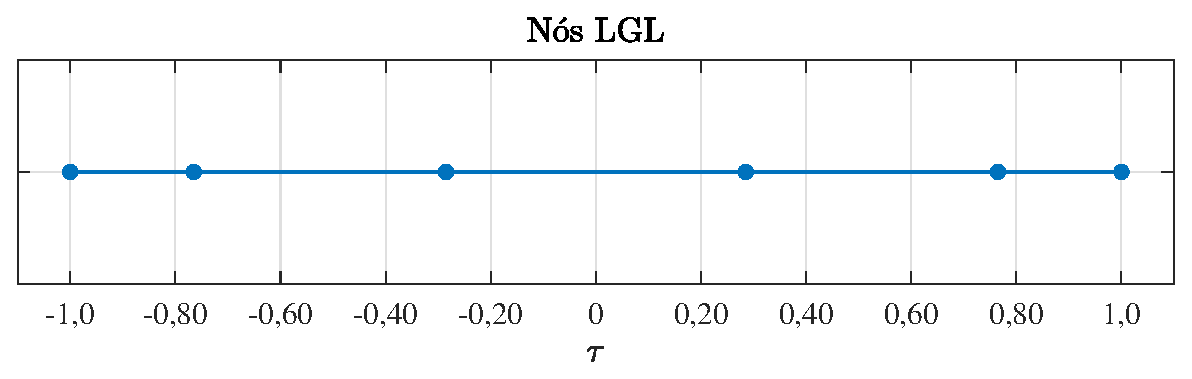
\includegraphics[width=1\linewidth]{fig/revisao/nosLGL}
	\captionof{figure}[Representação dos nós LGL]{Nós LGL para $ M = 5 $.}
	\label{fig:revisao:nosLGL}
	\vspace{\onelineskip}
\end{minipage}

Cabe ressaltar que a adoção do nós LGL possibilita que os estados e controles sejam aproximados com maior precisão e que as operações de derivação e integração associadas a essas variáveis sejam computadas de forma mais acurada. Se outro tipo de polinômio fosse empregado na interpolação dos estados e controles, como por exemplo o polinômio de Chebyshev, uma metodologia distinta seria adotada na determinação dos nós de colocação \cite{becerra_tutorial_2010}.

Como dito anteriormente, os estados e controles são aproximados pelo somatório de polinômios de Legendre no intervalo $ \tau \in [-1, \, 1] $. Além disso, é nesse mesmo intervalo que os nós LGL são definidos. No entanto, tanto os estados quanto os controles devem assumir valores em $ t \in [t_0, \, t_f] $. Assim sendo, conclui-se que a implementação da colocação pseudo-espectral depende da mudança de domínio descrito pela seguinte relação \cite{becerra_tutorial_2010}:
%
\begin{equation}
	\label{eq:revisao:mudancaDominioPseudoEspectral}
	\tau \leftarrow \frac{2}{t_f - t_0} t - \frac{t_f + t_0}{t_f - t_0}
\end{equation}
%

Neste caso, o PCO considerando esta abordagem pode ser formulado como segue \cite{becerra_psopt_2019}:
%
\begin{subequations}
\begin{equation}
\label{eq:revisao:PCOPseudoEspectral}
\underset{\mathbf{u}(\tau)}{\text{min}} \; J = \varphi \big( \mathbf{x}(1), 1 \big) + \frac{t_f - t_0}{2} \int_{-1}^{1} L \big( \mathbf{x}(\tau), \mathbf{u}(\tau), \tau \big) \, d\tau
\end{equation}
\vspace{-0.2cm}
\begin{equation}
\mathbf{\dot{x}}(\tau) = \frac{t_f - t_0}{2} \, \mathbf{f} \big( \mathbf{x}(\tau), \mathbf{u}(\tau), \tau \big), \; \mathbf{x}(-1) = \mathbf{x_0}
\end{equation}
\vspace{-0.7cm}
\begin{equation}
\mathbf{x_L} \leq \mathbf{x}(\tau) \leq \mathbf{x_U}
\end{equation}
\vspace{-0.7cm}
\begin{equation}
\mathbf{u_L} \leq \mathbf{u}(\tau) \leq \mathbf{u_U}
\end{equation}
\vspace{-0.7cm}
\begin{equation}
\mathbf{c}(\mathbf{x}(\tau), \mathbf{u}(\tau), \tau) \leq \mathbf{0}
\end{equation}
\vspace{-0.7cm}
\begin{equation}
{\bm \psi}(\mathbf{x}(1), 1) \leq \mathbf{0} 
\end{equation}
\end{subequations}

Então, para que a colocação pseudo-espectral de Legendre seja implementada, cada estado $ x(t) $ associado a $ \mathbf{x}(t) $ e cada controle $ u(t) $ associado a $ \mathbf{u}(t) $ devem ser aproximados segundo as seguintes relações:
%
\begin{subequations}
\begin{equation}
\label{eq:revisao:pseudoEspectral:estadosControles}
x(\tau) \approx \sum_{k = 0}^{M} x(\tau_k) \phi_k(\tau)
\end{equation}
\vspace{-0.15cm}
\begin{equation}
u(\tau) \approx \sum_{k = 0}^{M} u(\tau_k) \phi_k(\tau) 
\end{equation}
\end{subequations}
%
sendo $ \tau_k $ o $ k $-ésimo nó LGL e $ \phi_k(\tau) $ o $ k $-ésimo polinômio interpolador de Lagrange \cite{becerra_tutorial_2010}:
%
\begin{equation}
	\label{eq:revisao:pseudoEspectral:interpoladorLagrange}
	\phi_k(\tau) = \frac{1}{M(M+1) L_M(\tau_k)} \frac{(\tau^2 - 1) \dot{L}_M(\tau)}{\tau - \tau_k}
\end{equation} 

\todo[inline, size=normalsize, color=pink]{Falar de como a integral $ \int L dt $ é aproximada e de como as derivadas dos estados são aproximadas}

A integral de $L$ é computada empregando-se a quadratura de Gauss:
%
\begin{equation}
	\int_{-1}^{1} L \big( \mathbf{x}(\tau), \mathbf{u}(\tau), \tau \big) \, d\tau \approx \sum_{k=0}^{M} L(\tau_k) w_k
\end{equation}
%
sendo $ w_k $ um peso definido como \cite{becerra_tutorial_2010}:
%
\begin{equation}
	w_k = \frac{2}{M(M+1)} \frac{1}{L_N^2(\tau_k)}
\end{equation}

Vale ressaltar que $ L_M $ e $ L $ representam, respectivamente, o polinômio de Legendre de ordem $ M $ e o integrando associado ao termo de Lagrange da função objetivo $ J $. Dada a semelhança entre as notações atribuídas a essas grandezas, é preciso cuidado para que não haja confusões. 

A computação das derivadas dos estados nos nós de colocação é baseada na definição da matriz de diferenciação $ D $: 
%
\begin{equation}
	D_{ki} = \left\{
	\begin{array}{cl}
		\dfrac{L_M(\tau_k)}{(\tau_k - \tau_i)L_M(\tau_i)} & \text{se } k \neq i \vspace{0.25cm} \\
		-\dfrac{M(M+1)}{4} & \text{se } k = i = 0 \vspace{0.25cm}\\
		\dfrac{M(M+1)}{4} & \text{se } k = i = N \vspace{0.25cm} \\
		0 & \text{nos demais casos} 
	\end{array}
	\right.
\end{equation}  
%
e depende dos valores atribuídos aos estados em cada nó de colocação de forma que:
%
\begin{equation}
	\label{eq:revisao:aproximacaoDerivadas}
	\dot{x}(\tau_k) \approx \sum_{i=0}^{M} D_{ki} \, x(\tau_k)
\end{equation}
%

É possível ainda que a relação acima seja reescrita na forma matricial \cite{becerra_tutorial_2010}:
%
\begin{equation}
	\begin{bmatrix}
		\dot{x}(\tau_0) \\
		\dot{x}(\tau_1) \\
		\vdots \\
		\dot{x}(\tau_M) 
	\end{bmatrix} = 
	\begin{bmatrix}
		D_{00} & D_{01} & \cdots & D_{0M} \\
		D_{00} & D_{01} & \cdots & D_{0M} \\
		\cdots & \cdots & \ddots & \vdots \\
		D_{M0} & D_{M1} & \cdots & D_{MM} 
	\end{bmatrix}
	\begin{bmatrix}
		x(\tau_0) \\
		x(\tau_1) \\
		\vdots \\
		x(\tau_M) 
	\end{bmatrix}
\end{equation}

Assim sendo, $ M $ restrições de igualdade algébricas são formuladas como segue:
%
\begin{equation}
\mathbf{\dot{x}}(\tau_k) - \frac{t_f - t_0}{2} \, \mathbf{f} \big( \mathbf{x}(\tau_k), \mathbf{u}(\tau_k), \tau_k \big) = 0, \hspace{0.25cm} k = 0, \, \dots, \, M-1
\end{equation}
%
em que a derivada pode ser computada pela Eq. \eqref{eq:revisao:aproximacaoDerivadas}.

Assim como foi apresentado anteriormente, as restrições laterais, terminais, e de caminho podem ser reescritas como \cite{becerra_psopt_2019}: 
%
\begin{subequations}
\begin{equation}
\mathbf{x_L} \leq \mathbf{x}(t) \leq \mathbf{x_U} \rightarrow \mathbf{x_L} \leq \mathbf{x}(\tau_k) \leq \mathbf{x_U}, \; k = 0, \, \dots, \, M
\end{equation}
\vspace{-0.85cm}
\begin{equation}
\mathbf{u_L} \leq \mathbf{u}(t) \leq \mathbf{u_U} \rightarrow \mathbf{u_L} \leq \mathbf{u}(\tau_k) \leq \mathbf{u_U}, \; k = 0, \, \dots, \, M
\end{equation}
\vspace{-0.75cm}
\begin{equation}
\mathbf{c}(\mathbf{x}(t), \mathbf{u}(t), t) \leq \mathbf{0} \rightarrow \mathbf{c}(\mathbf{x}(\tau_k), \mathbf{u}(\tau_k), \tau_k) \leq \mathbf{0}, \; k = 0, \, \dots, \, M 
\end{equation}
\vspace{-0.75cm}
\begin{equation}
{\bm \psi}(\mathbf{x}(t_f), t_f) \leq \mathbf{0}  \rightarrow {\bm \psi}(\mathbf{x}(1), 1) \leq \mathbf{0} 
\end{equation}
\end{subequations}
%
em que a condição inicial é dada como:
%
\begin{equation}
\mathbf{x}_k = \mathbf{x_0}, \hspace{0.25cm} k = 0 
\end{equation}
%

Em resumo, para esta abordagem, o PCO é descrito como:
%
\begin{subequations}
\begin{equation}
\underset{\mathbf{u}(\tau_k), \, \mathbf{x}(\tau_k)}{\text{min}} \; J = \varphi \big( \mathbf{x}(1), 1 \big) + \frac{t_f - t_0}{2} \sum_{k=0}^{M} L(\tau_k) w_k 
\end{equation}
\vspace{-0.15cm}
\begin{equation}
\mathbf{\dot{x}}(\tau_k) - \frac{t_f - t_0}{2} \, \mathbf{f} \big( \mathbf{x}(\tau_k), \mathbf{u}(\tau_k), \tau_k \big) = 0, \hspace{0.25cm} k = 0, \, \dots, \, M
\end{equation}
\vspace{-0.7cm}
\begin{equation}
\mathbf{x}(-1) = \mathbf{x_0}
\end{equation}
\vspace{-0.7cm}
\begin{equation}
\mathbf{x_L} \leq \mathbf{x}(\tau_k) \leq \mathbf{x_U}, \hspace{0.25cm} k = 0, \, \dots, \, M 
\end{equation}
\vspace{-0.7cm}
\begin{equation}
\mathbf{u_L} \leq \mathbf{u}(\tau_k) \leq \mathbf{u_U}, \hspace{0.25cm} k = 0, \, \dots, \, M 
\end{equation}
\vspace{-0.7cm}
\begin{equation}
\mathbf{c}(\mathbf{x}(\tau_k), \mathbf{u}(\tau_k), \tau_k) \leq \mathbf{0}, \hspace{0.25cm} k = 0, \, \dots, \, M
\end{equation}
\vspace{-0.7cm}
\begin{equation}
{\bm \psi}(\mathbf{x}(1), 1) \leq \mathbf{0} 
\end{equation}
\end{subequations}
%
considerando que $ t_0 $ e $ t_f $ sejam conhecidos. Não sendo esse o caso, devem-se adotar $ t_0 $ e $ t_f $ como variáveis de projeto, e as restrições:
%
\begin{subequations}
\begin{equation}
t_{0L} \leq t_0 \leq t_{0U}
\end{equation}
\vspace{-0.85cm}
\begin{equation}
t_{fL} \leq t_f \leq t_{fU}
\end{equation} 
\end{subequations}
%
devem ser incorporadas ao PPNL, sendo os limites inferiores de $ t_0 $ e $ t_f $ denotados por $ t_{0L} $ e $ t_{fL} $ e os superiores por $ t_{0U} $ e $ t_{fU} $, respectivamente. 

%
%Uma vez que o PPNL tenha sido resolvido e que tanto $ \mathbf{x}(\tau_k) $ quanto $ \mathbf{u}(\tau_k) $ tenham sido determinados para $ k = 0, \, 1, \, \dots, \, M $, pode-se elaborar as trajetórias de estados e controle pelo implementação direta de \eqref{eq:revisao:pseudoEspectral:estadosControles}.

Considerando $ M = 2 $ e um estado e um controle pode-se escrever:
%
\begin{subequations}
\begin{equation}
x(\tau) = \sum_{k=0}^{2} x(\tau_k) \phi_k(\tau) = x(\tau_0) \phi_0(\tau) + x(\tau_1) \phi_1(\tau) + x(\tau_2) \phi_2(\tau)
\end{equation}
\vspace{-0.3cm}
\begin{equation}
u(\tau) = \sum_{k=0}^{2} u(\tau_k) \phi_k(\tau) = u(\tau_0) \phi_0(\tau) + u(\tau_1) \phi_1(\tau) + u(\tau_2) \phi_2(\tau) 
\end{equation}
\end{subequations}

Sabendo que $ M = 2 $, tem-se: 
%
\begin{subequations}
\begin{equation}
L_2(\tau) = \frac{3}{2} \tau^2 - \frac{1}{2}
\end{equation}
\vspace{-0.4cm}
\begin{equation}
\frac{L_2(\tau)}{d\tau} = 3 \tau
\end{equation}
\end{subequations}

Nesse caso, os nós de colocação LGL são dados por 
%
\begin{subequations}
\begin{equation}
\tau_0 = -1 
\end{equation}
\vspace{-0.75cm}
\begin{equation}
\tau_1 = 0
\end{equation}
\vspace{-0.75cm}
\begin{equation}
\tau_2 = 1
\end{equation}
\end{subequations}
%
enquanto os polinômios interpoladores de Lagrange são definidos como:
%
\begin{subequations}
\begin{equation}
\phi_0(\tau) = \frac{1}{2} (\tau^2 - \tau)
\end{equation}
\vspace{-0.6cm}
\begin{equation}
\phi_1(\tau) = 1 - \tau^2
\end{equation}
\vspace{-0.6cm}
\begin{equation}
\phi_2(\tau) = \frac{1}{2} (\tau^2 + \tau)
\end{equation}
\end{subequations}

Desta forma, segue que:
%
\begin{subequations}
\begin{equation}
\label{eq:revisao:estadosControlesInterpolados}
x(\tau) = a_x \, \tau^2 + b_x \, \tau + c_x 
\end{equation}
\vspace{-0.75cm}
\begin{equation}
u(\tau) = a_u \, \tau^2 + b_u \, \tau + c_u 
\end{equation}
\end{subequations}
%
em que: 
%
\begin{subequations}
\begin{equation}
a_x = \frac{x(\tau_0)}{2} - x(\tau_1) + \frac{x(\tau_2)}{2}
\end{equation}
\vspace{-0.3cm}
\begin{equation}
b_x = \frac{x(\tau_2)}{2} - \frac{x(\tau_0)}{2}
\end{equation}
\vspace{-0.5cm}
\begin{equation}
c_x = x(\tau_1)
\end{equation}
\end{subequations}
%

Analogamente:
%
\begin{subequations}
\begin{equation}
a_u = \frac{u(\tau_0)}{2} - u(\tau_1) + \frac{u(\tau_2)}{2} 
\end{equation}
\vspace{-0.3cm}
\begin{equation}
b_u = \frac{u(\tau_2)}{2} - \frac{u(\tau_0)}{2}
\end{equation}
\vspace{-0.5cm}
\begin{equation}
c_u = u(\tau_1)
\end{equation}
\end{subequations}

Apesar das expressões que descrevem $ x(t) $ e $ u(t) $ não terem sido formuladas, é possível que os valores atribuídos a essas grandezas para um dado $ t = t'$ sejam computados com base na determinação do $ \tau = \tau' $ correspondente, sendo que:
%
\begin{equation}
	\tau' = \frac{2}{t_f - t_0} t' - \frac{t_f + t_0}{t_f - t_0}
\end{equation}

Alternativamente, é possível que as expressões que descrevem $ x(t) $ e $ u(t) $ sejam de fato determinadas. Para tanto, é necessário que:
%
\begin{subequations}
\begin{equation}
x(t) = a_x' \, t^2 + b_x' \, t + c_x'
\end{equation}
\vspace{-0.85cm}
\begin{equation}
u(t) = a_u' \, t^2 + b_u' \, t + c_u' 
\end{equation}
\end{subequations}
%
sendo:
%
\begin{subequations}
\begin{equation}
a_x'= \frac{4}{(t_f - t_0)^2} \, a_x
\end{equation}
\vspace{-0.2cm}
\begin{equation}
b_x' = \frac{2}{t_f - t_0} \, b_x - 4 \frac{t_f + t_0}{(t_f - t_0)^2} \, a_x
\end{equation}
\vspace{-0.2cm}
\begin{equation}
c_x' = c_x - \frac{t_f + t_0}{t_f - t_0} b_x + \frac{(t_f + t_0)^2}{(t_f - t_0)^2} a_x
\end{equation}
\end{subequations}
%

Analogamente:
%
\begin{subequations}
\begin{equation}
a_u' = \frac{4}{(t_f - t_0)^2} \, a_u
\end{equation}
\vspace{-0.2cm}
\begin{equation}
b_u' = \frac{2}{t_f - t_0} \, b_u - 4 \frac{t_f + t_0}{(t_f - t_0)^2} \, a_u
\end{equation}
\vspace{-0.2cm}
\begin{equation}
c_u' = c_u - \frac{t_f + t_0}{t_f - t_0} b_u + \frac{(t_f + t_0)^2}{(t_f - t_0)^2} a_u
\end{equation}
\end{subequations}

Independente da abordagem utilizada, fica evidente que computar $ x(t) $ e $ u(t) $ com base nos resultados advindos do emprego da colocação pseudo-espectral não é uma tarefa trivial. De fato, a elaboração das trajetórias de estados e controles a partir dos resultados provenientes da implementação das colocações trapezoidal ou Hermite-Simpson é baseada em um procedimento consideravelmente mais simples e direto. No entanto, uma vez que um único polinômio é utilizado na interpolação de cada um dos estados e controles, as trajetórias associadas à colocação pseudo-espectral tendem a ser bastante suaves.  

\todo[inline, size=normalsize, color=pink]{Falar dos PCOs multifásicos}
  
\todo[inline, size=normalsize, color=pink]{Pacotes utilizados (descrição sucinta com as principais características e link pra download do código fonte e do guia do usuário) }

\section{Pacotes avaliados}

O estudo comparativo apresentado no presente trabalho baseia-se no emprego dos pacotes $ PSOPT $, do $ FALCON $ e do $ COPILOTS $. Vale ressaltar que a utilização desses não depende do pagamento de qualquer licença, e que tanto o $ PSOPT $ quanto o $ COPILOTS $ são pacotes de código aberto. Cada um dos pacotes avaliados é sucintamente descrito a seguir. 

\subsection{\boldmath$ PSOPT $}

O $ PSOPT $ (\textit{Pseudospectral Optimal Control Solver}) é um pacote desenvolvido para solução de PCOs a partir do emprego de métodos pseudo-espectrais, mas que possibilita a utilização de métodos de discretização local, como a colocação trapezoidal e a colocação Hermite-Simpson \cite{becerra_psopt_2019}. Escrito em C++, apresenta um desempenho bastante satisfatório em comparação com outros pacotes baseados no Matlab\textsuperscript{\textregistered} \cite{becerra_psopt_2010}. Tem sido largamente empregado pela comunidade científica e foi uma das ferramentas utilizadas no planejamento da primeira missão espacial brasileira rumo ao espaço profundo, em direção ao sistema de asteroides 2001-SN263 \cite{becerra_psopt_2010}. Além disso, o código fonte do $ PSOPT $ conta com inúmeros exemplos e um guia do usuário bastante completo, que traz instruções referentes à utilização do pacote e introduz conceitos fundamentais acerca da colocação pseudo-espectral. O desenvolvimento do presente trabalho baseia-se na versão 4.0 do $ PSOPT $ cujo código fonte, que só pode ser compilado em sistemas Linux ou Mac, pode ser acessado em \url{https://cutt.ly/OjYG7hD}.

\subsection{\boldmath$ FALCON $}

O $ FALCON $ (\textit{FSD Optimal Control Toolbox for Matlab\textsuperscript{\textregistered}}) é um pacote desenvolvido para a solução de PCOs a partir do uso de métodos de colocação direta como a trapezoidal e o método de Euler. Esse pacote faz uso de ferramentas de cálculo simbólico na obtenção das derivadas analíticas da função objetivo e das restrições, o que proporciona um desempenho bastante satisfatório em termos do tempo de processamento. Apesar do $ FALCON $ ser um pacote de código fechado que possui uma versão paga, vale ressaltar que, empregando-se a versão gratuita, já é possível resolver a maioria dos PCOs. Aqueles que desejarem utilizar o $ FALCON $ devem criar uma conta em \url{https://cutt.ly/6jYBzcE} e enviar aos desenvolvedores uma mensagem solicitando o acesso ao código fonte. O guia do usuário do $ FALCON $, em contrapartida, pode ser acessado em \url{https://cutt.ly/RjYBEee} por qualquer um que se interesse em utilizar o pacote \cite{rieck_falconm_2020}.

\textcolor{red}{Arthur, o $ COPILOTS $ é metolologia, por isso eu retirei daqui e coloquei no próximo capítulo}.

\section{Métricas para a Avaliação de Pacotes Computacionais}

%\todo[inline, color=pink, size=normalsize]{Dificuldades de se comparar pacotes e quais métricas são comumente utilizadas e dificuldade de escolher os estudos de caso}

A realização de um estudo comparativo (ou \textit{benchmarking}) de pacotes computacionais é normalmente motivada pela necessidade de verificarem-se as deficiências associadas a cada pacote, de forma que os devidos aprimoramentos possam ser implementados \cite{dolan_benchmarking_2002}. Além disso, os dados advindos de um estudo desse tipo podem ser bastante úteis aos usuários, que passam a ter uma noção mais acertada das capacidades de cada pacote \cite{bongartz_numerical_1997, parejo_metaheuristic_2012}. 

No geral, um estudo comparativo de pacotes computacionais desenvolvidos para solução de problemas de otimização (POs) é baseado em dois principais critérios: desempenho e confiabilidade \cite{benson_interior-point_2000}. O primeiro deles diz repeito à qualidade da solução atribuída a um dado pacote, avaliada a partir do valor ótimo da função objetivo, da máxima violação das restrições, ou do atendimento das condições de otimalidade. Estão ainda associados ao desempenho, parâmetros relacionados ao processo de obtenção da solução, como o número de avaliações da função objetivo, o número de nós de colocação, o tempo de processamento, ou o número de iterações 
%
\cite{bongartz_numerical_1997, mittelmann_benchmarking_1998, dolan_benchmarking_2004, darby_hp-adaptive_2011, gruning_feedforward_2012, wang_optimal_2013, luis_tiago_de_freixo_ramos_numerical_2014, garcia-heras_comparison_2014, bock_evaluation_2016, baines_benchmark_2019, foroozandeh_numerical_2019, howell_altro_2019}. 
%
Já a robustez diz respeito à probabilidade de um dado pacote resolver um PO qualquer, independentemente da qualidade da solução. A robustez pode ser medida, por exemplo, pela razão entre o número de execuções bem sucedidas e o número total de execuções, sendo cada execução empregada na resolução de um PO distinto \cite{betts_performance_1993, bongartz_numerical_1997}. 

Cabe ressaltar que métricas mais sofisticadas podem ser propostas. Um exemplo são os chamados perfis de desempenho, propostos em \citeonline{dolan_benchmarking_2002_online}, que são funções de distribuição que possibilitam a determinação da probabilidade de um dado pacote resolver um estudo de caso até então não avaliado, ou da probabilidade desse mesmo pacote se sair melhor do que outros no tocante a uma determinada métrica. Além disso, utilizando apenas a representação gráfica dos perfis de desempenho, é possível comparar diferentes pacotes de forma simples e direta. No entanto, não é recomendado que os perfis de desempenho sejam empregados na comparação de poucos pacotes ou na avaliação de um pequeno número de estudos de caso. Em \citeonline{dolan_benchmarking_2002_online}, por exemplo, é utilizado um banco de dados contendo 70 estudos de caso. 

Pode-se ainda empregar a métrica proposta em \citeonline{benson_interior-point_2000}, que possibilita que pacotes sejam comparados aos pares. Considerando, por exemplo, a comparação entre os pacotes A e B, e assumindo $ t_{pA} $ e $ t_{pB} $ como sendo os tempos de processamento associados a esses pacotes, respectivamente, define-se $ r = t_{pA}/t_{pB} $. Em seguida, computa-se o $ r $ associado a cada um dos $ n_p $ estudos de caso em análise e, por fim, determina-se $ r_s = \dfrac{1}{n_p} \sum_{i=1}^{n_p} r$. Caso $ r_s < 1 $, pode-se dizer que, em média, os tempos de processamento associados ao pacote A são menores que aqueles atribuídos ao pacote B. O problema dessa abordagem é que ela possibilita apenas que os pacotes sejam comparados aos pares, de forma que fica difícil empregá-la quando há um número muito grande de pacotes sendo avaliados. Além disso, recomenda-se que $ n_p $ seja consideravelmente alto. Em \citeonline{benson_interior-point_2000}, por exemplo, adota-se $ n_p = 889 $.

Uma outra alternativa, no caso dos métodos diretos, seria comparar a solução obtida à solução analítica \cite{darby_hp-adaptive_2011}. No entanto, obter a solução analítica de um PCO pode ser uma tarefa bastante difícil, e algumas vezes até impossível, principalmente se a formulação desse PCO incluir muitas restrições, dinâmicas complexas, ou múltiplas fases. 

Há ainda métricas que não estão associadas diretamente às soluções obtidas por meio do emprego do pacote em análise, que não podem ser quantificadas, ou que tem caráter subjetivo. Algumas dessas métricas podem ser representadas pelas seguintes questões: 
\begin{itemize}
	\item O pacote é de fácil utilização?
	\item O pacote exige uma licença paga? 
	\item Quais plataformas (Windows\textsuperscript{\textregistered}, Linux, Mac\textsuperscript{\textregistered}) suportam o pacote? 
	\item O código-fonte do pacote segue as boas práticas de programação? 
	\item O pacote é amplamente utilizado pelos membros da comunidade científica? 
	\item Com que frequência o pacote recebe atualizações? 
	\item A documentação associada ao pacote é completa? 
	\item O pacote possui uma comunidade de usuários ativa? 
	\item Como é o suporte fornecido pelos desenvolvedores do pacote?
\end{itemize} 

Diante do que foi apresentado, fica evidente que determinar as métricas a serem avaliadas em um estudo comparativo não é uma tarefa trivial. Ainda assim, as conclusões advindas da computação dos dados obtidos por meio de um estudo comparativo depende fortemente das métricas utilizadas. Uma vez que há vários tipos de métricas e que é difícil afirmar que uma seja melhor do que outra, bem como é complicado dizer quais métricas devem ser empregadas \cite{bongartz_numerical_1997}. Além do mais, essa escolha pode ter uma relação direta com a aplicação à qual está vinculada a solução do PCO em análise. Pode ser, por exemplo, que uma aplicação \textit{online} requira baixos tempos de processamento, de forma que essa métrica se torne uma das mais importantes no contexto em questão \cite{febbo_nloptcontrol_2020}. 

Além disso, há outros fatores que tornam a implementação de um estudo comparativo uma tarefa bastante complexa. Primeiramente, como já foi mencionado, é necessário que um conjunto de estudos de caso extenso e heterogêneo seja considerado, o que faz com que a representação dos dados obtidos se torne um desafio. Dada a extensão do conjunto de estudos de caso, pode ser necessário que os dados advindos do estudo comparativo sejam tratados estatisticamente, porém, uma vez que há várias formas de fazê-lo, a interpretação desses dados é fonte de discordância \cite{dolan_benchmarking_2002, bongartz_numerical_1997}. 
